\documentclass[titlepage]{article}
\usepackage[bottom=3cm, right=2cm, left=2cm, top=3cm]{geometry}
\usepackage{graphicx}
\usepackage{hyperref}
\usepackage{float}
\restylefloat{table}
\usepackage{amsmath}
\usepackage{booktabs}

\title{SFWRENG 4NL3 Assignment 4: \\ Pretrained Transformers}
\author{Sumanya Gulati}
\date{1 April 2025}

\begin{document}

\begin{titlepage}
    \maketitle
\end{titlepage}

\newpage 

\tableofcontents
\listoftables
\listoffigures

\newpage

\section{Dataset}
For this assignment, I am using the GoEmotions dataset extracted from the HuggingFace can be accessed 
\href{https://huggingface.co/datasets/google-research-datasets/go_emotions}{here}. The task at hand 
involves emotion classification, aiming to identify and categorize the emotions expressed in textual data. This 
is essential for applications such as sentiment analysis, mental health assessment, enhancing human-computer 
interactions and more. \\

The GoEmotions dataset comprises of about 58,000 English Reddit comments, each annotated for 27 distinct emotion 
categories or marked as neutral. The simplified version of the dataset with predefined train, val and test splits 
has been used for this assignment. 

\subsection{Data Collection}
The dataset has been constructed by selecting English-language comments from Reddit by researchers at Amazon Alexa, 
Google Research and Stanford Linguistics. A complete list of authors can be found \href{https://arxiv.org/abs/2005.00547}
{here}. The comments were extracted from Reddit using a variety of automated methods along with data curation techniques 
such as reducing profanity, length filtering, sentiment and emotion balancing, masking and more. Further information 
about the data collection process can be found in section 3.1 of \href{https://arxiv.org/pdf/2005.00547}{this paper}.

\subsection{Dataset Structure}
Each instance of the dataset corresponds to a reddit comment with an ID and one or more emotion annotations including neutral.
The simplified configuration of the dataset which has been used for this assignment, includes:

\begin{itemize}
    \item \texttt{text}: the Reddit comment
    \item \texttt{labels}: the emotional annotations
    \item \texttt{comment\_id}: a unique identifier for the comment
\end{itemize}

The input for the task is a Reddit comment in English and the corresponding output is a set of one or more labels corresponding 
to the 27 emotion categories or neutral, reflecting the emotional content of the comment.

The labels are stored as a list of integers ranging from 0 to 27 where each integer represents an emotion category or neutral. The 
label mapping is as follows:

\begin{table}[H] \label{tab:labels}
    \centering
    \begin{tabular}{lll}
    \toprule
    \textbf{Label Number} & \textbf{Label Category} \\
    \midrule
    0 & admiration \\
    1 & amusement \\
    2 & anger \\
    3 & annoyance \\
    4 & approval \\
    5 & caring \\ 
    6 & confusion \\
    7 & curiosity \\
    8 & desire \\
    9 & disappointment \\
    10 & disapproval \\
    11 & disgust \\
    12 & embarrassment \\
    13 & excitement \\
    14 & fear \\
    15 & gratitude \\
    16 & grief \\
    17 & joy \\
    18 & love \\
    19 & nervousness \\
    20 & optimism \\
    21 & pride \\
    22 & realization \\
    23 & relief \\
    24 & remorse \\
    25 & sadness \\
    26 & surprise \\
    27 & neutral \\
    \bottomrule
    \end{tabular}
    \caption{Label Mapping}
\end{table}

\subsection{Evaluation Metrics}
The following evaluation metrics have been used to assess the performance of the BERT-based model:
\begin{itemize}
    \item Model Performance:
        \begin{itemize}
            \item Emotion-level Precision, Recall, F1: Measured per each emotion in the GoEmotions taxonomy.
            \item Transfer Learning: F1 score on data transferred between domain X and GoEmotions.
        \end{itemize}
    \item Deciison thresholds: No thresholds are used. The data is presented in full granularity.
    \item Uncertainty and variability: Repeated experiments have yielded results with similar taxonomical rankings.
\end{itemize}

The model has been evaluated on 10 publicly available datasets including 9 benchmark datasets presented in compilation 
by \href{https://aclanthology.org/C18-1179/}{Bostan and Klinger} and the \href{https://github.com/google-research/google-research/tree/master/goemotions}
{GoEmotions} eval set. Full details about the evaludation results can be found in the \href{https://arxiv.org/pdf/2005.00547}{paper}.

\subsection{Data Splits}
The dataset is divided into training, validating and test splits as follows:

\begin{table}[H] \label{tab:data_split}
    \centering
    \begin{tabular}{lll}
    \toprule
    \textbf{Data Split} & \textbf{Number of Instances} \\
    \midrule
    Training & 43,410 \\
    Validation & 5,426 \\
    Test & 5,427 \\
    \bottomrule
    \end{tabular}
    \caption{Data Split Overview}
\end{table}

Class distributions for the training and test splits are shown in the figure \ref{fig:class_distribution}.

\begin{figure}[H] \label{fig:class_distribution}
    \centering
    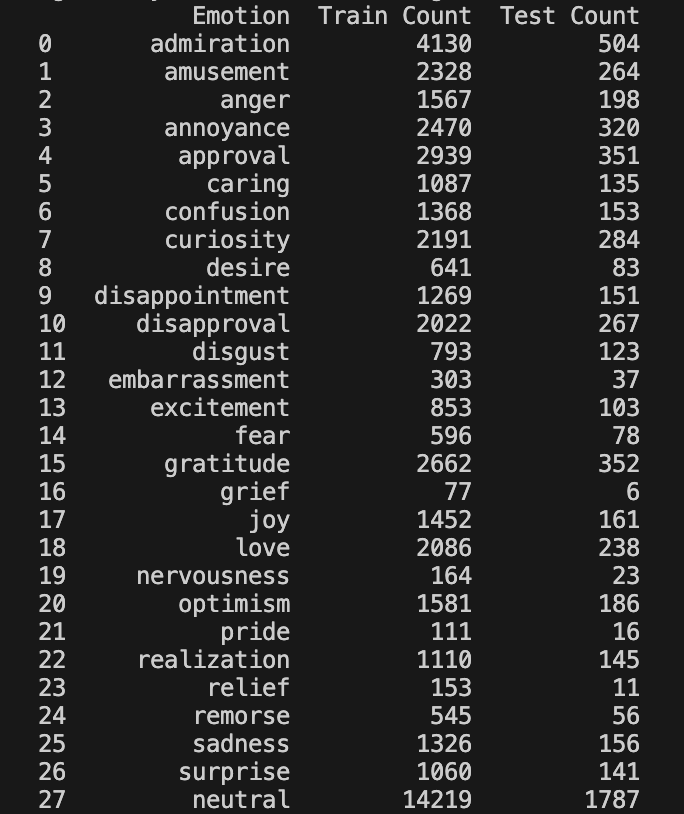
\includegraphics[scale=0.8]{/Users/sg/Desktop/courses/winter-2025/4nl3/assignments/assignment-4/homework4_report/figures/class_distributions.png}
    \caption{Class Distribution in Training and Test Splits}
\end{figure}

\subsection{Additional Features}
Although the comments vary in length, the maximum sequence length has been capped at 30 tokens in the training and evaludation datasets 
to ensure concise and focused emotional expressions. Furthermore, linguistic context consistency has been ensured by only choosing comments 
that are in English.
 








\section{Methodology}
% Describe the steps that you performed and what informed your decisions.
% For example, if you decided not to lowercase the text because it gave better results at a later
% stage, include that decision and your reasoning for doing that. This should include details
% of your preprocessing steps, e.g. lowercasing, stemming, not just saying “each document was
% preprocessed”. Describe the kind of analysis you performed. For any steps that you did not
% implement yourself (e.g. topic modeling), you should mention which package/library was
% used.

\subsection{Preprocessing}
Since the \texttt{data\_extract.py} file only extracts the data from the PDF and store it in a text file, 
the first step in preprocessing the dataset was to clean the text. This was accomplished using the following 
methods through iterative testing:
\begin{itemize}
    \item Replacing all new lines with a blank space.
    \item Removing all words that have a hyphen followed by a blank space. For example, long- term to longterm.
    \item Removing all leading and trailing spaces along with the replacement of multiple blank spaces with a single space.
    \item Removing all digits to streamline the frequency count and ranking of alphabetic tokens. This was implemented 
    because with the digits in the corpus, the years and other random numbers referencing legal cases and such populated the 
    top 10/top 25 counts corrupting the data analysis.
    \item Removing all punctuation for more accurate tokenization.
\end{itemize}

\subsubsection{Naive-Bayes}
Further preprocessing for Naive-Bayes included the following steps:
\begin{itemize}
    \item Using the list of common stopwords from the \textsl{nltk} library to remove words that do not reflect the 
    actual content.
    \item The list of stopwords was expanded to account for commonly found words in the dataset that did not convey the 
    sentiment or the content of the sentence. This includes words such as \texttt{said, would, one, jan, feb}.
    \item To further refine our results, commonly used legal jargon was also added to the list of stopwords. This includes
    words such as \texttt{hearings, committee, senator, judge, case}.
\end{itemize}

\subsubsection{Latent Dirichlet Allocation (LDA) Preprocessing}
Further preprocessing for LDA included the following steps:
\begin{itemize}
    \item Adding additional stop words including `sgpohearings' and `sgpohearingstxt' that are not actual words with defined meanings.
    \item Using NLTK's lemmatizer removing any tokens starting with `sgpo'.
\end{itemize}

\subsection{Bag-of-Words Representation}
As shown in tutorials, the \texttt{CountVectorizer()} function was used to implement Bag-of-Words on the dataset.
Probability calculations given in the instructions PDF for this assignment were then used to implement the 
\texttt{calculate\_word\_probabilities()} function. The output from this function was then to calculate the 
Log Likelihood Ratio. 

\subsection{Naive-Bayes Model}

Given the fact that the dataset is made up of real transcripts of legal hearings, the used of names of the judges and/or
the senators interviewing them are over-represented in the dataset. This skews the results of analyses performed 
on the processed dataset. \\

To combat this issue and to maintain the focus on the goal of this assignment, classifications were establish so the focus of 
the analyses would remain on words that align with the characteristics of the nominee. 4 different classifications - 
Legal Interpretation, Background Experience, Personal Characteristics and Competency Qualification were created. \\

Each of these classifications was populated with a list of related words that speak to that particular classification, such as - 
words like `ruling', `precedent', `principle', `rights' and more were added to the Legal Interpretation classification. By analyzing the 
frequency of these words in the vocabulary for the female and male nominees, any potential bias towards a nominee can be spotted. If 
the focus of the hearing is on 1-2 classifications as opposed to a general overview of all of them, this would highlight implicit bias.

\subsection{Topic Modelling}
The \texttt{gensim} and \texttt{pyLDSvis} libraries were used to implement LDA topic modelling as shown in the tutorial. 
The \texttt{get\_topic\_words()} and \texttt{get\_document\_topic()} functions were then used to get information on the topics and 
documents.  

\subsection{Experimentation}
In addition to importing all the functions from the \texttt{processing.py} file, two new functions were added to implement text normalization 
variation and LDA variation. \texttt{PorterStemmer()} was used to implement stemming as a part of the preprocessing of the data. Another function 
was then implemented to create a TF-IDF matrix using the \texttt{TfidfVectorizer()} function. The code for this was based on the tutorials.

\section{Results and Analysis}
% Present your results as formatted tables and figures. You should
% have at least one table or figure for each of 2.3, 2.4, and 2.5. This must include at least the
% results of the required steps, but may also include any interesting findings you came across
% (e.g. results of topic modeling with and without a given preprocessing step that made a
% difference in the quality of the results). For each table and figure, include a description of
% your main takeaways.
The results and insights gather from the analyses has been summarized in the following subsections.

\subsection{Naive-Bayes}

\begin{table}[H] \label{tab:naive-bayes}
    \centering
    \begin{tabular}{llll}
    \toprule
    \textbf{Gender} & \textbf{Category} & \textbf{Word} & \textbf{LLR Score} \\
    \midrule
    female & background experience & backgrounds & 1.931906639972084 \\
    female & background experience & experienced & 1.0156159080979297 \\
    female & background experience & experiences & 1.9682742841429581 \\
    female & background experience & framework & 2.52789007207838 \\
    female & background experience & services & 1.4982706548972224 \\
    \midrule
    female & personal characteristics & biases & 1.6645918703447364 \\
    female & personal characteristics & ethnicity & 2.6250538205320293 \\
    female & personal characteristics & gender & 1.0750667224516768 \\
    female & personal characteristics & genderbased & 2.10180567676748 \\
    female & personal characteristics & grace & 1.2751271035830118 \\
    female & personal characteristics & identity & 1.1209764237557547 \\
    \midrule
    female & competency qualification & applicability & 1.8941663119892365 \\
    female & competency qualification & availability & 1.46928311802397 \\
    \midrule
    male & legal interpretation & judicially & 1.1407866747180364 \\
    male & legal interpretation & overruling & 1.2014112965344719 \\
    \midrule
    male & background experience & practiced & 1.4245548478486825 \\
    male & background experience & worker & 1.0762481535804653 \\
    male & background experience & workload & 1.4817132616886308 \\
    \midrule
    male & personal characteristics & beliefs & 1.3067718121922978 \\
    male & personal characteristics & embraced & 1.7693953341404107 \\
    male & personal characteristics & unbiased & 2.0570774065921924 \\
    \midrule
    male & competency qualification & disability & 1.209779546204988 \\
    male & competency qualification & wellqualified & 2.0570774065921924 \\
    \bottomrule
    \end{tabular}
    \caption{Results from the Naive-Bayes Analysis}
\end{table}

As shown in table \ref{tab:naive-bayes}, the analysis shows that when interviewing female nominees are interviewed, greater focus 
is put on their personal characteristics with conversations about biases, gender, grace and identity taking up a significant amount 
of attention. In terms of their background experiences and competency qualifictaions, the focus is put on their availability and 
the top words from the category across documents are neutral in tone. None of the words added to the legal interpretation category 
were found in a significant frequency for the female nominees. \\

As for the male nominees, however, words like `judicially' and `overruling' are highlighted showing the focus on the conversation around 
the nominee's career in law and their judgments. The conversations around personal characteristics seem to be more focused on the 
individual as opposed to their gender or other aspects of their identity. The most starking difference can be seen in the tone of 
the competency qualifications since the word `wellqualified' seems to have a very high probability showing the appreciative tone 
of the hearings.

\subsection{Topic Modelling}

The complete list of topic words along with their labels can be found in the \texttt{topic\_words.csv} file. The averages for the top 
20 of these topics split by the gender can also be found in the \texttt{category\_topics.csv} file. 

\begin{figure}[H]\label{fig:LDA}
    \centering
    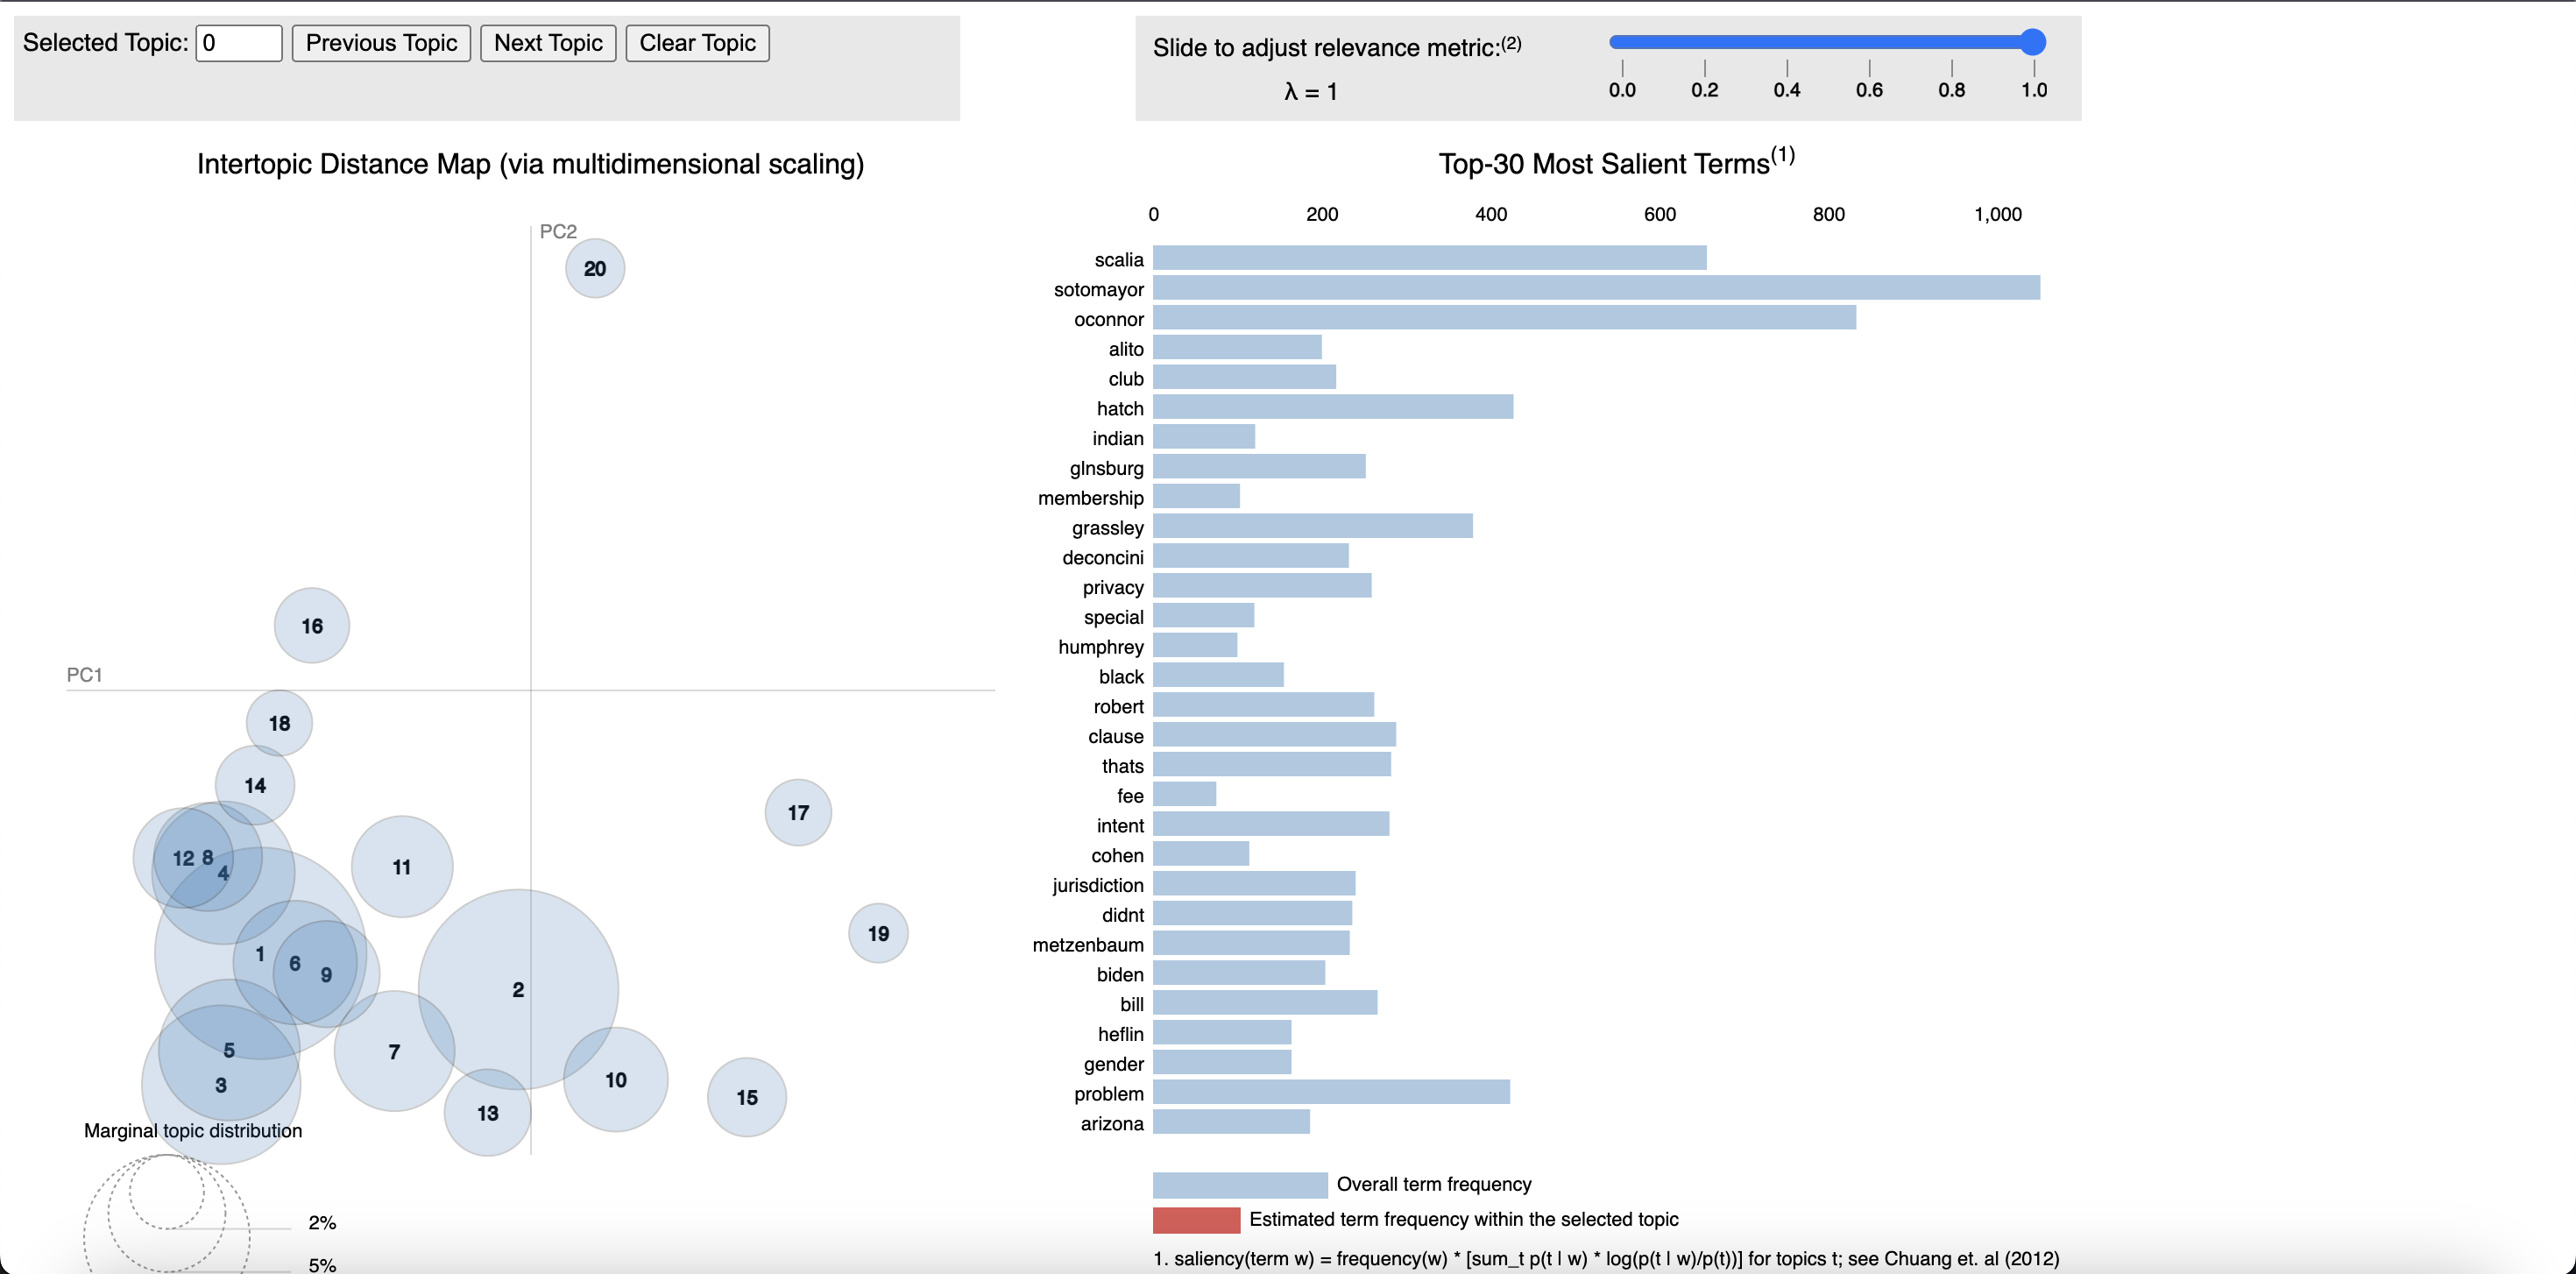
\includegraphics[scale=0.35]{/Users/sg/Desktop/courses/winter-2025/4nl3/assignments/assignment-2/dataset/visualizations/LDA.png}
    \caption{Results from LDA Topic Modelling}
\end{figure}

As shown in figure \ref{fig:LDA}, the intertopic distance map visualizes the relationship between the different topics where each bubble represents 
a topic with the bubble's size indicating the topic's overall prevalence in the dataset. Topics 12, 8, 4, 1, 6, 9, 5, 3 and more are overlapping and 
clustered together suggesting similarity. \\

The 30 most important words are either names, identity-related terms (gender, black) or general legal jargon. A few interesting insights have been listed here:
\begin{itemize}
    \item Topic 12 that mentions Justice Ginsburg and legislation is much more popular along female nominees given the work she has done championing women's rights 
    and gender equality.
    \item The use of words such as `business' and `agency' are significantly more popular with male nominees showing the focus on the nominee's competencies and
    judicial philosophies. This also includes top 15 where talks of legal jurisdictions with words such as `privacy', `clause' and `national' are way more popular 
    with male nominees. This is supported by the arrangement of the thematic clusters for topics 5, 15, 8 and 11.
    \item The thematic clusters show topics 3, 12, 2 and 13 that focus on Justice Ginsburg, Justice O'Connor,gender and voting legislation are more heavily focused on 
    privacy and reproductive rights, often regarded as `women`'s issues`.
\end{itemize}

\subsection{Experimentation}
\begin{figure}[H] \label{fig:stemming}
    \centering
    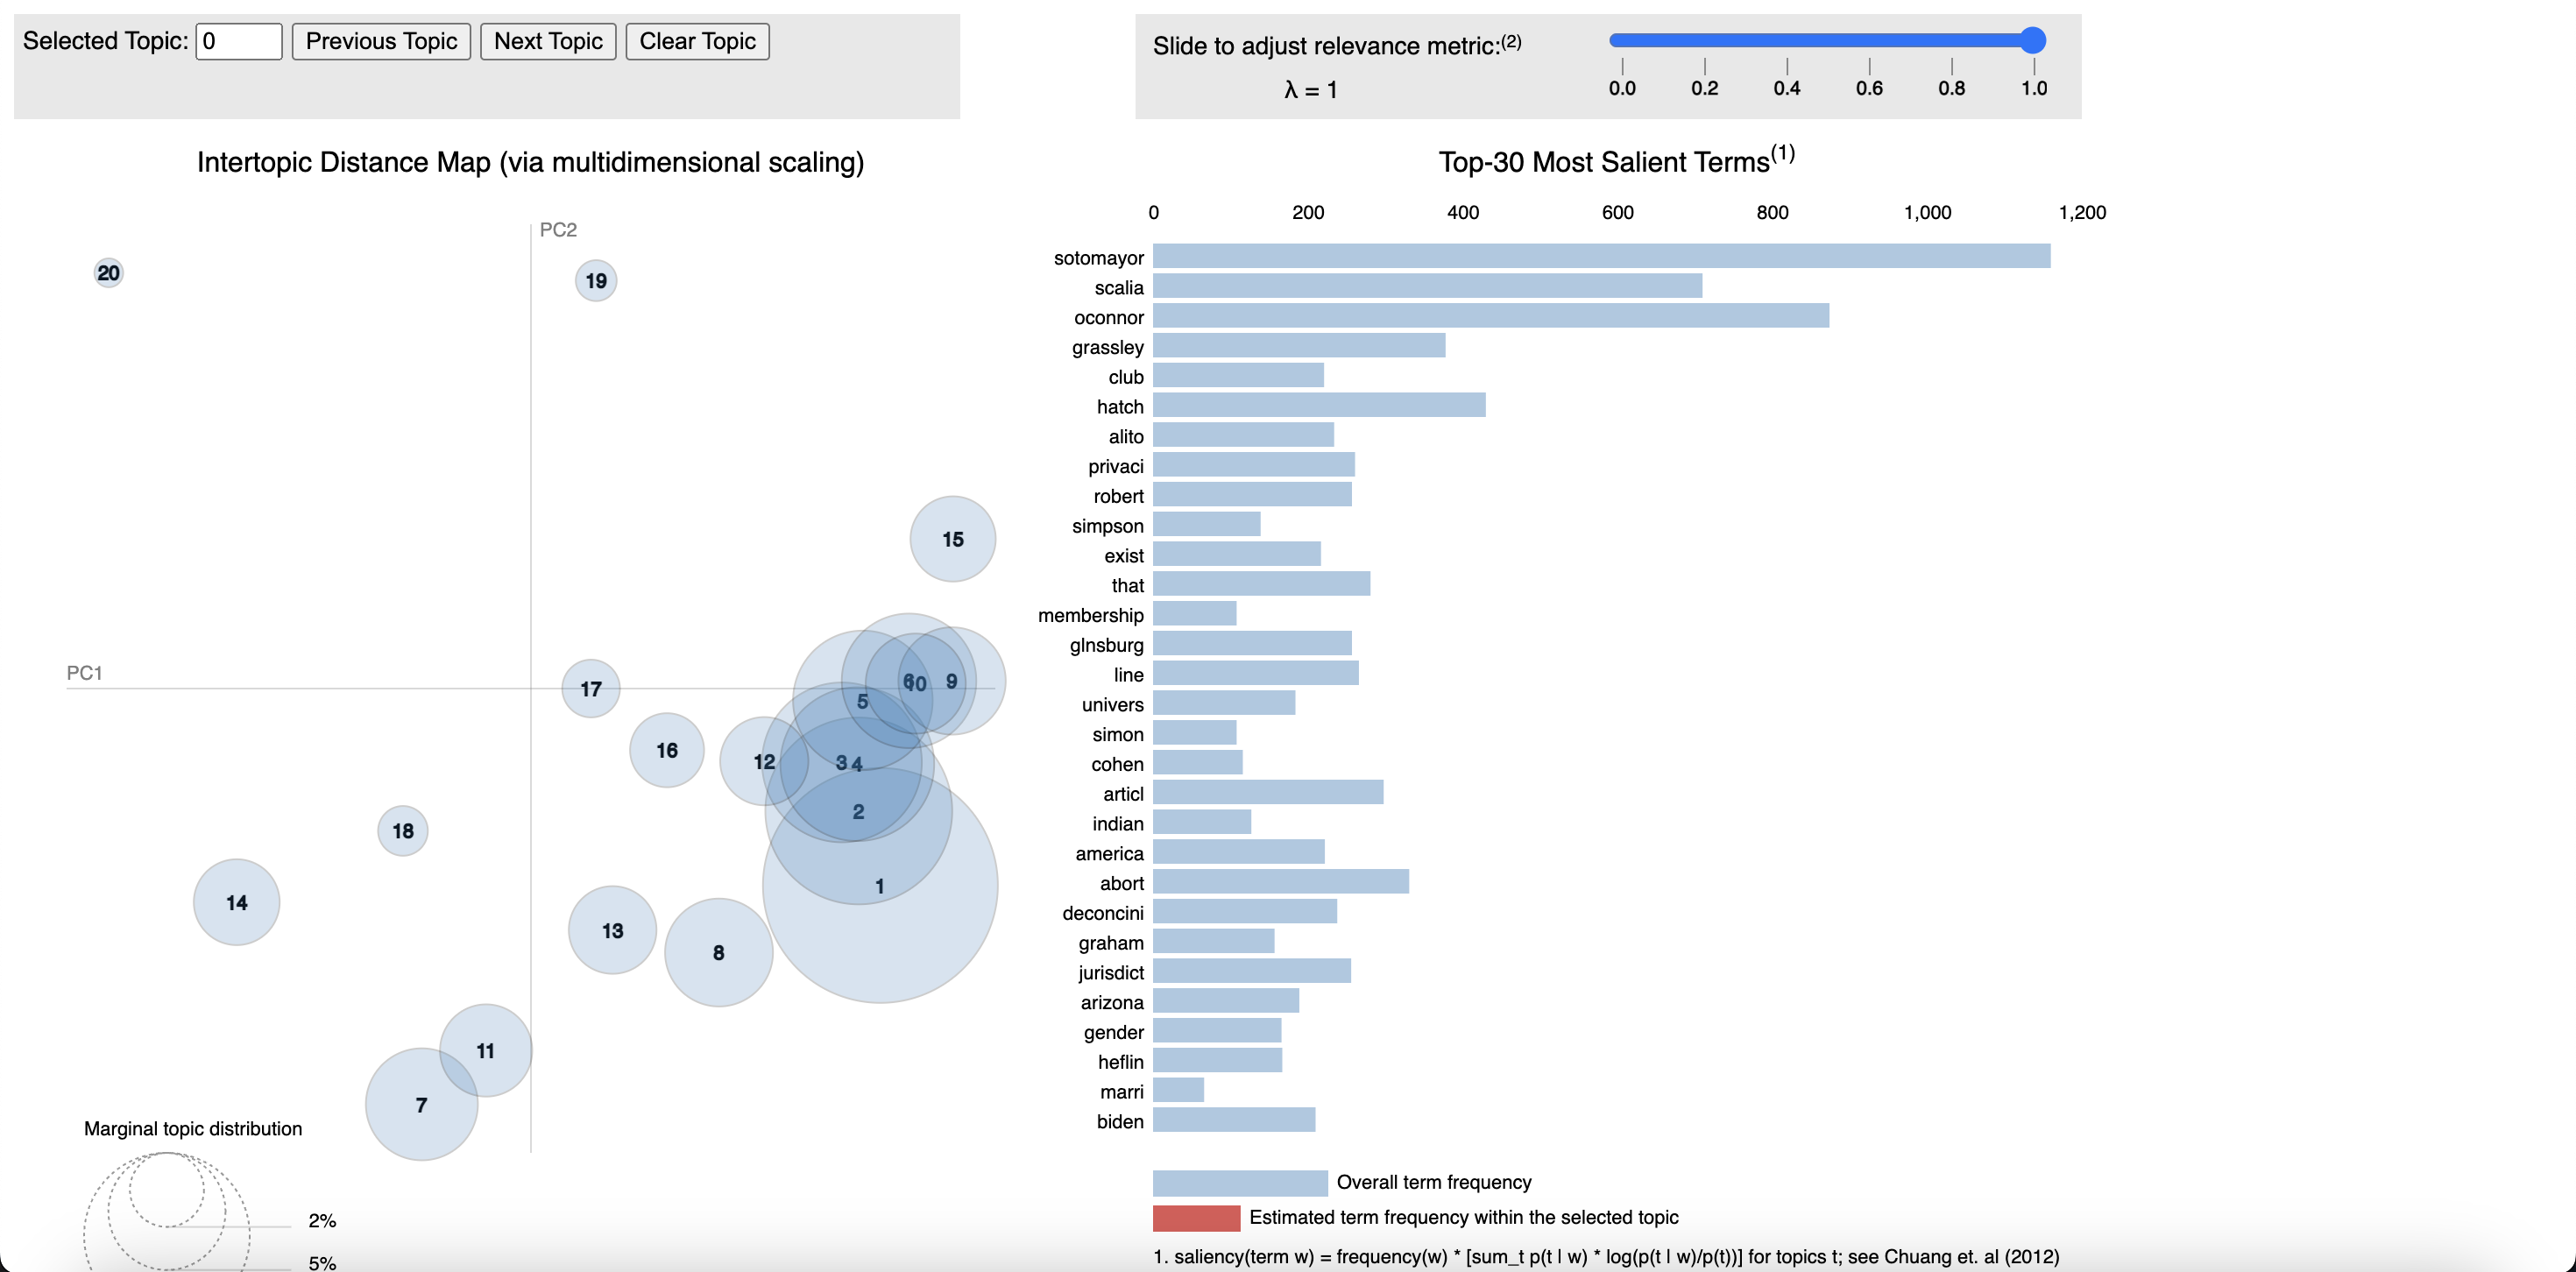
\includegraphics[scale=0.35]{/Users/sg/Desktop/courses/winter-2025/4nl3/assignments/assignment-2/dataset/visualizations/stemming_LDA.png}
    \caption{Results from LDA Topic Modelling Post-Stemming and with TF-DIF}
\end{figure}

As shown in figure \ref{fig:stemming}, it is obvious that stemming has been used as terms like `privacy' have been incorrectly spelt as `privaci'.
The analysis result is pretty similar to the previous section's result excluding the misspelt words.

\section{Discussion}

This section outlines common findings and insights dervided from the program.

\subsection{Findings}
% Include two subsections in the discussion. The first should talk about what
% you learned about your dataset. Imagine that you are describing what your results showed,
% at a high level, to a friend who does not have any NLP experience but is interested in the
% corpus that you chose.
As outlined in the description of the dataset, the hypothesis remains proven true. The Naive-Bayes analysis and the LDA analysis support the theory 
that when interviewing women nominees, more focus is placed on their personal characteristics and questioning their qualifications as opposed to the male 
nominees who are questioned over their judicial philosophy and appreciated for their competency and qualifications.  For instance, topics involving privacy 
rights, gender, and specific legal clauses appeared more frequently in female discourse, while topics involving procedural aspects or judiciary figures had 
a higher presence in male discourse.

\subsection{Reflection}
% The second subsection should cover what lessons you personally
% learned during the completion of the assignment. You might write about how you found and
% processed the data, preprocessing effects on downstream analysis, topic modeling results,
% limitations of your approaches, or other interesting aspects that were new to you.
Although I was aware of the importance of text normalization and preprocessing, their importance became a lot more evident during the course of this assignment. Even small 
changes in preprocessing steps altered the topic distributions, which highlighted the sensitivity of topic modeling to text cleaning procedure. It was also surprising 
(although should have been expected) that the transcripts are dominated by names and judicial jargon. \\

It has also become clear to me that topic modelling has limitations such as the fact that it provides a useful high-level overview of themes, it lacks the ability to 
capture nuanced contextual meanings. Some topics were too broad or contained words that seemed unrelated at first glance. Overall, this assignment deepened my understanding 
of text analysis and the complexities involved in extracting meaningful insights from unstructured textual data. It also reinforced the importance of critical interpretation 
when working with computational models - numbers alone do not tell the full story and human judgment is essential in deriving meaningful conclusions.

\end{document}